\section{Privacy}

% //TODO: Write why he need privacy
Privacy is a very useful and beneficial feature in payment systems. First and foremost, payment activities involve some sensitive personal information. Users usually do not want this information to be disclosed in order to protect their personal information, as it can be used to discriminate against individuals based on their financial history or purchasing habits. 

Apart from the protection of personal data, the lack of privacy raises concerns in other areas as well ~\cite{SoKPrivacyPreservingComputing}.
It also has a negative impact on fairness by enabling front-running attacks ~\cite{FronRrunningAttacks}. In these attacks, a malicious individual monitors the transactions of other users and races to issue his own transaction, aiming to have it confirmed first. An example could be racing to win an auction by exploiting this advantage. It can also create "tainted" currency. That is, coins that no one wants to own because they are associated with an undesirable coin history, such as being part of an illegal trade.

The first level of privacy used by Bitcoin and most existing cryptocurrencies is pseudonymity. In this approach, transactions hide neither the participants nor the values transferred. Privacy relies on pseudonymous addressing, which aims to break the link between the addresses of the system and the identities of real users. Payment systems that use the permissionless setting allow and encourage users to have more than one such pseudonym. However, even this provides a very weak anonymity guarantee. Various de-anonymization attacks have been proposed in the literature ~\cite{meiklejohn2013fistful}, ~\cite{reid2013analysis}, ~\cite{ron2013quantitative}, ~\cite{tschorsch2016bitcoin}, based on clustering by analyzing either the inputs and outputs of the transactions or the behavior of the users ~\cite{SoKAnonymityInCryptocurrencies}.

Stronger privacy guarantees include the following properties: confidentiality and anonymity. Confidentiality hides the transaction amounts, while anonymity hides the pseudonyms of the real participants in a transaction. There are two levels of anonymity, set anonymity and full anonymity. In set anonymity, the user's identity is either one of $n$ possible identities, where $n$ is the size of the set. Full anonymity is provided when the participants can be any user of the system.

\begin{figure}
    \centering
    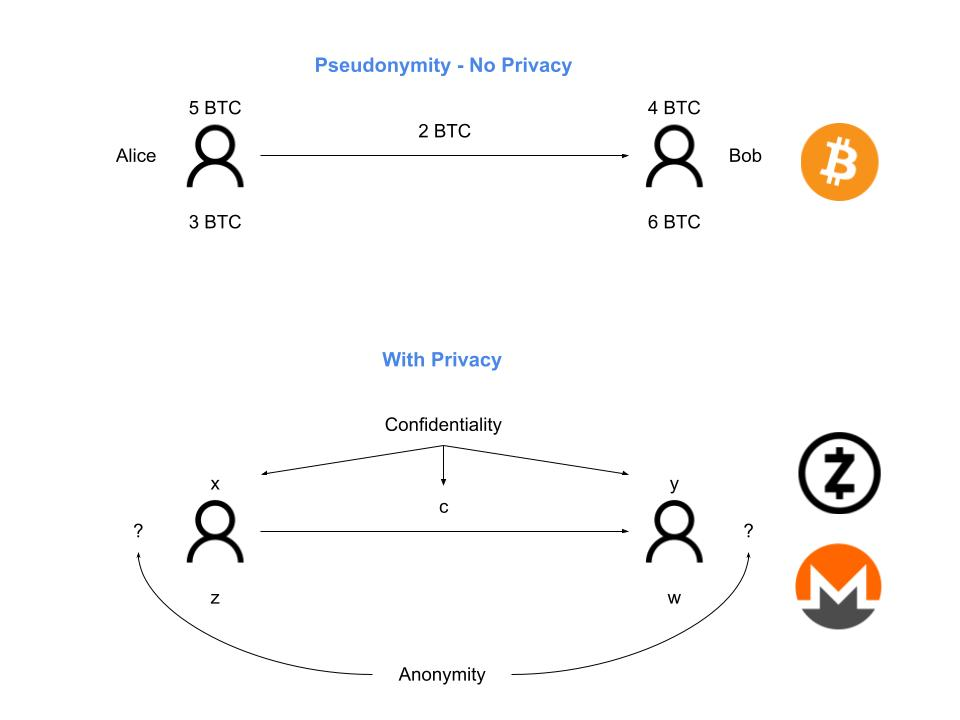
\includegraphics[width=0.9\textwidth]{images/privacy/Anonymity in blockchain.jpg}
    \caption{Privacy in Payment Systems}
    \label{fig:privacy_img}
\end{figure}

% The basic idea behind implement privacy in the payment systems are the following:
% \begin{itemize}
%     \item Hide transaction values inside
%         \textbf{commitments} (confidentiality).
%         \item Use \textbf{Anonymity Set} to disguise the real participants in the tx (anonymity).
%         \item Provide \textbf{ZK-Proofs} for the validity of tx.
% \end{itemize}

To implement privacy properties, private payment systems use the following basic idea: 
\begin{itemize}
    \item confidentiality is achieved through homomorphic commitments, which aim to hide the amounts transacted as well as the values of users' accounts. 
    % if an account-based scheme is used, 
    \item Anonymity is achieved through anonymity sets (e.g., shielded pools, ring signatures) that hide the pseudonyms of the real participants in a transaction.
\end{itemize} 
In addition, a necessary tool for private payment systems is zero-knowledge proof, which aims to ensure the validity of transactions without revealing the above information.